% !TEX root = ../main.tex



\chapter{预备章节}
\section{K\"ahler 流形}
一个Hermitian流形$(X,g)$是一个复流形$X$配上一个和其复结构$I$相容的黎曼度量$g$，相容即是指
\[
g(\cdot,\cdot)=g(J(\cdot),J(\cdot))
\]
将$X$看成实流形我们将其切丛记为$T_X$，其复化被复结构分裂成
\[
T_X\otimes \C=T^{1,0}\oplus T^{0,1}
\]
特别的$(T_X,I)$与$T^{1,0}$存在自然同构
\[ 
v\to \frac{1}{2}(v-iI(v))
\]
相对应的，对于复化的$k$-形式丛我们有
\[
\Omega_X^k=\bigoplus_{p+q=k}\Omega_X^{p,q}
\]
$g$可以诱导一个$(1,1)$-形式$\omega\coloneqq g(I(\cdot),\cdot)$。若$\omega$是闭形式，则称$(X,g)$为K\"ahler流形。由于$\omega$可以还原出$g$，我们也可将其记为$(X,\omega)$。

同时$g$可以诱导出$(T_X,I)$上的Hermitian度量
\[
h\coloneqq g-i\omega
\]
我们将$g$的复化记为$g_{\C}$，需注意，将其限制在$T^{1,0}$上我们有
\[g_{\C}=\frac{1}{2}h\]
在局部坐标$z=(z^1,\cdots,z^n)$下，我们有
\[
h=h_{i\bar{j}}\diff z^i\otimes \diff \overline{z}^j\quad \omega=\frac{i}{2} h_{i\bar{j}}z^i\otimes \diff \overline{z}^j
\]

在$\Omega_X^\bullet$上，我们定义Lefschetz算子$L\coloneqq \cdot\wedge \omega$。
由于$g_{\C}$诱导了$\Omega_X^\bullet$上的内积，我们有自然的伴随算子，将其记为$\Lambda$。在局部坐标下若有$(1,1)$-形式$\eta=\eta_{i\bar{j}}dz^i\wedge d\overline{z}^j$，我们有
\[
\Lambda\eta=\frac{2}{i}h^{\bar{i}j}\eta_{i\bar{j}}
\]
特别的对于光滑函数$f$，
\[
-2i\Lambda \partial\overline{\partial}f=\Delta_g f \footnote{在本篇文章中，我们约定Laplace算子为$\Delta=-\Div\cdot \nabla f$。}
\]

\section{抛物丛起源}
全纯向量丛上的抛物结构最早应出自\cite{Me-Se}。文章作者通过研究平坦向量丛在非紧黎曼面上的无穷远渐进行为获得了抛物结构。本小节将简单介绍抛物结构的来源以及定义抛物结构的动机。

令 $G\subset \PSU(2,\R)$ 是一个离散子群，使得它自由地作用于上半平面$\HH$且其商空间是有限体积的。令$\HH^+=P\cup \HH$其中$P$为群作用的抛物点，则$X=\HH^+/G$是一个紧黎曼面。给定一个$n$维厄米特向量空间$V$以及一个酉表示$\rho: G\to \GL(n,V)$, 我们得到一个带$G$作用的向量丛$E=\HH\times V$. 我们总是可以通过共轭变换将抛物点变到无穷远点，因此我们只考虑抛物点为无穷远点的情况。令$y\in P$ 是$X$上的一个抛物尖点，则对于$\delta$充分大，存在一个邻域$\U_y=\HH_\delta/G_\infty$, 其中$\HH_\delta\coloneqq \{z=x+iy\in \HH|y>\delta\}$, $G_\infty$由一个抛物元素$T:z\mapsto z+a$生成，其中$a\in \R$，为简单起见我们取$a=1$。

由以上设定，我们考虑丛$E$限制在$\HH_\delta$上的$G$不变的有界全纯截面，即有界全纯映射$F:\HH^+_\delta\to \HH^+_\delta\times V$其形式为$F(z)=(z,f(z))$并且满足$f(z+1)=\rho(T)\cdot f(z)$. 在合适的酉标架$\{e_i\}_i$下，$\rho(T)$可以被对角化为
\[
\rho(T)=
\begin{pmatrix*}
    \exp(2\pi i \alpha_1) & &\\
    & \ddots & \\
    & & \exp(2\pi i \alpha_n)
\end{pmatrix*}
\]
其中$0\leq \alpha_i\leq\alpha_{i+1}<1$。则在该酉标架下$f=(f_i)_i$满足$f_i(z+1)=\exp(2\pi i \alpha_i)f_i(z)$，通过直接计算可得$f_i(z)=\exp(2\pi i \alpha_i z)g_i(\tau)$ 其中$\tau=\exp(2\pi i z)$, $g_i$ 是去心圆盘上的全纯函数。由于$f$是有界的，因此$g_i$在$\tau=0$处也是全纯的。

基于以上观察，我们可以在紧黎曼面$X$上定义局部自由层$\pE$，其定义如下：我们把$\HH^+$到$X$的商映射记成$q$, 对于不与抛物点相交的开集$\U$，$\pE(\U)=E^G(q^{-1}(\U))$, 其中$E^G$表示$G$不变的全纯截面。对于包含抛物点$y$的开集$\U_y$, $\pE(\U_y)$则由上述讨论的$G$不变的有界全纯截面组成。上述讨论表明，${\pE}_{,y}$ 是秩为$n$的${\OX}_{,y}$自由模，其生成元为$F_i: z\to \exp(2\pi i \alpha_i z)e_i$，因此$\pE$是局部自由层，我们也可以认为$\pE$是紧黎曼面$X$上的向量丛。

基于$V$上的度量，我们有$|F_i|=O(|\tau|^{-\alpha_i})$，因此我们可以基于这些生成元的收敛速度在$y$处对该向量丛的纤维$W_y$进行分层。将互不相同的$\alpha_i$从小到大记为$\{\alpha_j\}_j$, 令$F_jW_{y}\coloneqq\{F_i||F_i|\geq |\tau|^{-\alpha_j}\}$，我们得到一个递减的滤链
\[
 W_y=F_1W_{y}\supset F_2W_{y}\supset \cdots \supset F_lW_{y}\supset F_{l+1}W_{y}=0
\]
对于每个$F_jW_y$我们赋予权重$\alpha_j$, 从而得到一个带权的滤链。
我们称该带权滤链为向量丛$\pE$在$y$处的抛物结构。对于包含多个抛物点的情况，我们可以在每个抛物点处定义类似的滤链，从而得到一个全局的抛物结构。

引入抛物结构的目的在于记录原始向量丛$E$在无穷远点处的渐近行为，从而尽可能多的保留原始向量丛$E$的信息。事实上，我们有以下结论：
\begin{proposition}
    假设$E_1$，$E_2$是来自如上所述的两个$G$的酉表示产生的向量丛，则他们各自诱导抛物丛${\pE}_1$，${\pE}_2$。对任意的$G$等变态射$\phi: E_1 \to E_2$，它诱导了丛${\pE}_1$到${\pE}_2$的态射，不妨依旧记为$\phi$，并且在抛物点$y$处满足$\phi(F_iW_{1,y})\subset F_jW_{2,y}$当且仅当$\alpha_{1,i}>\alpha_{2,j}$。
\end{proposition}
因此记录抛物结构是有必要的。

以上的内容成为了抛物丛定义的动机。
% \section{脚注}
\section{Hodge丛}
由于本篇文章极大地受到了Simpson~\cite{Si1}的启发，在本预备章节的最后我们重新回顾~\cite{Si1}当中的结果。
\subsection{Hodge结构的形变}
考虑 $\phi: Y \to X$ 是一个极化 Kähler 流形的族。即存在 $\omega \in H^2(Y, \mathbb{Z})$，使得对于任意 $x \in X$，$\omega|_{Y_x}$ 是 Kähler 的。

在局部 $U_x \subset X$ 上，$Y$ 微分同胚于 $Y_x \times U_x$。考虑向量丛 $R^k\phi_* \mathbb{C} \otimes \mathcal{O}_X|_{U_x} \simeq H^k(Y_x, \mathbb{C}) \times U_x$。在此之上存在 Gauss-Manin 联络 $\nabla = d$。对于任意两根纤维 $H^k(Y_x, \mathbb{C}) \simeq H^k(Y_{x'}, \mathbb{C})$（通过基于 $\nabla=d$ 的平行移动诱导同构）。

Lefschetz 分解 $L: R^k\phi_* \mathbb{C} \xrightarrow{\cup [\omega]} R^{k+2}\phi_* \mathbb{C}$ 使得我们可以关注本原部分：
\[ R^k\phi_*\mathbb{C}_{\text{prim}} \otimes \mathcal{O}_X |_{U_x} \simeq H^k(Y_x, \mathbb{C})_{\text{prim}} \times U_x \]
在 $H^k(Y_x, \mathbb{Z})$ 上定义 $Q(\alpha, \beta) = <L^{n-k}\alpha, \beta>$，这与 $H^k(Y_x, \mathbb{Z}) \simeq H^k(Y_{x'}, \mathbb{Z})$ 的同构是兼容的。
因此，在向量丛 $R^k\phi_* \mathbb{C}_{\text{prim}} \otimes \mathcal{O}_X =: \mathcal{H}^k$ 上我们有一个 Hermitian 形式 $h(\alpha, \beta) \coloneqq i^{k} Q(\alpha, \bar{\beta})$，其关于 $\nabla$ 平行。

Hodge过滤 (Hodge filtration) 定义为 \[F^p H^k(Y_x, \mathbb{C}) = \oplus_{a \ge p} H^{a, k-a}(Y_x) \subset H^k(Y_x, \mathbb{C})\]
这给出了一个映射（局部）：
\[ \mathcal{P}^{k,p}: X \to G \subset \text{Gr}(k, p, H^k(Y_x, \mathbb{C})) \quad \text{(全纯)} \]
通过 $\mathcal{P}^{k,p}$ 拉回 $G$ 上的重言子丛 $S^{k,p}$，得到 $\mathcal{H}$ 的一个全纯子丛 $F^p\mathcal{H}$。

\textbf{Griffiths 横截性 (Griffiths transversality):}
\[ \nabla F^p \mathcal{H}^k \subset F^{p-1}\mathcal{H}^k \otimes \Omega_X^1 \]
这一性质诱导了一个全纯态射（无穷小 VHS 或 Higgs 场）：
\[ \theta: \mathcal{H}^{p,q} \to \mathcal{H}^{p-1, q+1} \otimes \Omega_X^1 \]
其中
\[
\mathcal{H}^{p,q} = F^p\mathcal{H}^k / F^{p+1}\mathcal{H}^k \simeq F^p\mathcal{H}^k \cap \overline{F^{k-p}\mathcal{H}^k}
\]
Griffiths 横截性给出了分解 $\nabla = \bar{\theta}_h + \partial_h + \bar{\partial} + \theta$。

\begin{definition}[极化Hodge结构 PVHS]
一个 PVHS 是一个 $C^\infty$ 丛 $(\oplus \mathcal{H}^{p,q}, \nabla)$ 存在Hermitian形式 $s = \oplus s^{p,q}$ （使得 $h = \oplus (-1)^p s^{p,q}$ 为度量），满足 $\nabla s = 0$。
\end{definition}

\begin{definition}[Hodge 丛系统]
一个 Hodge 丛系统是 $\oplus (\mathcal{H}^{p,q}, \bar{\partial})$ 配备 $\theta: \mathcal{H}^{p,q} \to \mathcal{H}^{p-1, q+1} \otimes \Omega_X^1$，满足 $\theta \wedge \theta = 0$（即无穷小 VHS）。
\end{definition}

\subsection{分析结果}

\begin{theorem}\label{th1}
假设 $(X, \omega)$ 满足 Simpson~\cite[Section 2]{Si1}的假设，且 $(E, \bar{\partial}, \theta, A, K)$ 是一个带有群作用 $A$ 和度量 $K$ 的 Higgs 丛，使得 $\Lambda F_{\nabla_K^{hs}}$ 有界，并且关于该群作用是稳定的。那么存在一个 $A$-不变度量 $H$，满足 $\det(H) = \det(K)$，与 $K$ 可比，$\bar{\partial}(K^{-1}H) \in L^2$，使得 $\Lambda F_{\nabla_H^{hs}}^\perp = 0$。
\end{theorem}

\begin{proposition}\label{prop3.3}
假设 $E$ 是一个 Higgs 丛，且 $H$ 是一个满足 $\Lambda F_{\nabla_H^{hs}}^\perp = 0$ 的度量。则
\[ \left( 2c_2(E, H) - \frac{r-1}{r} c_1(E, H)^2 \right) \cdot \omega^{n-2} = C \int_X \tr(F_{\nabla_H^{hs}}^\perp \wedge F_{\nabla_H^{hs}}^\perp) \wedge \omega^{n-2} \ge 0 \]
如果等号成立，则 $F^\perp = 0$。特别地，如果 $\tr(F)=0$ 且 $c_2(E, H) \cdot \omega^{n-2} = 0$，则 $\nabla_H^{hs}$ 是平坦的。
\end{proposition}

\subsection{VHS 的构造（向量丛版本）}

给定 $X$ 上的 Hodge 丛系统 $(\oplus_{p+q=k} \mathcal{H}^{p,q}, \theta)$，使得
\[ \theta: \mathcal{H}^{p,q} \to \mathcal{H}^{p-1, q+1} \otimes \Omega_X^1 \]
满足可积性条件 $\theta \wedge \theta = 0$，以及一个度量 $h = \oplus_{p+q=k} h^{p,q}$，我们可以构造一个 Hitchin-Simpson 联络 $\nabla_h^{hs} := \nabla_h^c + \theta + \theta^{*h}$，其中 $\nabla_h^c$ 是 $h$ 的 Chern 联络。
容易验证 $\nabla_h^{hs}$ 保持半双线性形式 $s := \oplus_{p+q=k} \sqrt{-1}^{q-p} h^{p,q}$。因此，如果曲率 $F_{\nabla_h^{hs}}$ 为零，我们就恢复了一个极化Hodge结构形变。

\begin{theorem}\label{th8.2}
假设 $(X, \omega)$ 是紧致 Kähler 流形。则Hodge结构形变的范畴（态射保持联络）同构于满足 $c_1(E)=0, c_2(E) \cdot [\omega]^{n-2} = 0$ 且为度数为零的稳定 Hodge 丛系统的直和的全子范畴。
\end{theorem}

\begin{proof}
如果 $E$ 是稳定且度数为零的，由 $\partial\bar{\partial}$-引理，我们可以在 $\det(E)$ 上找到一个度量 $h$ 使得 $F_{\nabla_h^{hs}}$ 是 $c_1(E)$ 的调和代表元，于是 $\Lambda F_{\nabla_h^{hs}} = 0$（注意对于线丛，Hitchin-Simpson 联络和 Chern 联络相同）。根据定理\ref{th1}，我们在 $E$ 上得到一个度量使得 $\Lambda F = 0$。如果 $E$ 在全子范畴中，我们对每个直和项做此操作。通过构造，$\tr(F)$ 是 $c_1(E)$ 的调和代表元，因此 $\tr(F)=0$。此时应用命题~\ref{prop3.3} 得到 $F=0$，即 $E$ 来自于一个Hodge结构形变。另一方面，如果 $E$ 来自 VHS，由 Chern-Weil 公式可知 $E$ 位于该子范畴中。

至此我们证明了该函子是满射。接下来证明它是全忠实的，即证明 VHS 范畴中的态射与 Hodge 丛系统范畴中的态射一一对应。单射是显然的，只需证明如果 $f: E' \to E''$ 是一个来自 VHS 范畴的 Hodge 丛系统映射，即 $E'$ 和 $E''$ 分别配备平坦联络 $\nabla'$ 和 $\nabla''$，则 $\nabla(f)=0$（其中 $\nabla$ 是 $\text{Hom}(E', E'')$ 上的诱导联络），或等价地 $f$ 保持联络。此处省略证明。实际上这是一个同构。假设从一个 VHS $(E, \nabla')$ 出发，使用定理\ref{th1} 得到 $E$ 上的平坦联络 $\nabla''$，上述论证表明 $\id: (E, \nabla') \to (E, \nabla'')$ 保持联络，即 $\nabla' = \nabla''$，因此它是同构。
\end{proof}

\subsection{VHS 的构造（主丛版本）}

\subsubsection*{Cartan 分解}

设 $\g_0$ 为实半单李代数，$\g$ 为其复化。$\g_0$ 的 Cartan 对合 $\theta$ 是一个对合自同构，使得双线性形式 $B_\theta(X, Y) := -B(X, \theta(Y))$ 是正定的，其中 $B$ 是 Killing 形式。我们有 Cartan 分解 $\g_0 = \mathfrak{k}_0 \oplus \mathfrak{p}_0$，其中 $\mathfrak{k}_0$ 和 $\mathfrak{p}_0$ 分别是 $\theta$ 特征值为 1 和 -1 的特征空间。复化后得到 $\g = \mathfrak{k} \oplus \mathfrak{p}$。

定义 $\tau := \sigma \circ \theta$，其中 $\sigma$ 是 $\g$ 关于 $\g_0$ 的复共轭。则 $h(X, Y) := -B(X, \tau(Y))$ 是 $\g$ 上的 Hermitian 度量。简单的计算表明 $h([Z, X], Y) = h(X, [-\tau(Z), Y])$，即 $Z^{h*} = -\tau(Z)$。

\subsubsection*{Hodge群 (Hodge group)}

考虑来自Hodge结构形变的结构群，它是 $GL(V)$ 的李子群 $G_0$，其中 $V$ 是带有Hodge结构 $V = \oplus_{p+q=k} V^{p,q}$ 的复向量空间。$G_0$ 的复化李代数 $\g := \g_0 \otimes \C$ 是 $\En(V)$ 的子代数，并继承了Hodge分解 $\g = \oplus_p \g^{p, -p}$ 使得 $[\g^{r, -r}, \g^{p, -p}] \subset \g^{p+r, -p-r}$。

\begin{definition}[极化Hodge群]
一个极化Hodge群 $G_0$ 是一个半单实代数李群，其复化李代数 $\g$ 容许一个Hodge分解 $\g = \oplus_p \g^{p, -p}$ 满足 $[\g^{r, -r}, \g^{p, -p}] \subset \g^{p+r, -p-r}$，且 Killing 形式 $B$ 保持Hodge分解（即若 $p+r \neq 0$ 则 $B(\g^{p, -p}, \g^{r, -r}) = 0$），并且满足 $(-1)^{p+1} B|_{\g^{p, -p}} > 0$。
\end{definition}

\subsubsection*{Hodge丛主系统 (Principal system of Hodge bundles)}

由 Cartan 分解的唯一性，可知 $\mathfrak{k} = \oplus_{p \text{ even}} \g^{p, -p}$ 且 $\mathfrak{p} = \oplus_{p \text{ odd}} \g^{p, -p}$。设 $K_0$ 为 $G_0$ 中使得 $\Ad(k)$ 保持Hodge分解的李子群。易证 $K_0$ 是紧致的。记 $K$ 和 $G$ 分别为 $K_0$ 和 $G_0$ 的复化。

\begin{definition}
一个Hodge丛主系统是一个全纯主 $K$-丛 $P$，连同一个全纯截面 $\theta \in H^0(P \times_K \g \otimes \Omega_X)$，其值仅取在 $\g^{-1, 1}$ 中，并且满足 $[\theta(u), \theta(v)] = 0$ 对任意 $u, v \in T_xX$ 成立。
\end{definition}

由于 $\Ad(k)$ 保持Hodge分解，我们也可以视 $\theta$ 为 $P \times_K \g^{-1, 1} \otimes \Omega_X$ 的全纯截面。
设 $P_H \hookrightarrow P$ 为结构群从 $K$ 到 $K_0$ 的 $C^\infty$ 约化。这可以看作 $P$ 上的一个度量 $H$。于是存在唯一的联络 $\nabla^c$ 在 $P_H$ 上与 $P$ 的全纯结构兼容。

\subsubsection*{主Hodge结构形变 (Principal variation of Hodge structure)}

$\g$ 上的极化诱导了一个 Hermitian 度量 $h$，进而诱导了伴随丛 $P_H \times_{K_0} \g$ 上的度量。逐点来看，假设 $\theta = Z \otimes dz$，定义
\[ \bar{\theta}_H := Z^{h*} \otimes d\bar{z} = -\tau(Z) \otimes d\bar{z} = \sigma(Z) \otimes d\bar{z} = \bar{\theta} \]
即 $\bar{\theta}_H$ 正是 $\theta$ 关于 $\g_0$ 和 $X$ 赋予的实结构的复共轭。于是 $\theta + \bar{\theta}_H$ 是 $P_H \times_{K_0} \g_0 \otimes A_X^1$ 的 $\g_0$-值光滑截面。这样一个截面自然诱导了主丛 $P_H \times G_0$ 上的张量形式。因此我们在主丛 $R_H := P_H \times G_0$ 上有一个合理的联络 $\nabla^{hs} = \nabla^c + \theta + \bar{\theta}_H$。

\begin{definition}
关于Hodge群 $G_0$ 的主Hodge结构形变是一个Hodge丛主系统 $(P, \theta)$ 连同一个度量 $P_H \hookrightarrow P$，使得诱导的联络 $\nabla^{hs}$ 是平坦的。
\end{definition}

\subsubsection*{齐性空间的切空间}

\begin{proposition}\label{tangentbundleofhomogeneouspace}
$T(G/K) \cong G \times_K (\g/\mathfrak{k})$，其中 $\g$ 和 $\mathfrak{k}$ 分别是 $G$ 和 $K$ 的李代数。
\end{proposition}

\begin{proof}
视 $G$ 为 $G/K$ 上的主 $K$-丛。令 $\pi: G \to G/K$ 为投影。在点 $gK$，我们可以通过映射 $d\pi_g$ 将 $\g/\mathfrak{k}$ 与 $T_{gK}(G/K)$ 等同。具体来说，对于 $X \in \g$ 和定义在 $G/K$ 上的函数 $f$（注意 $f$ 在 $K$ 的右作用下不变），有 $d\pi_g(X)(f) = \frac{d}{dt} f(g \cdot \exp(tX))$。显然 $\mathfrak{k}$ 是此映射的核。问题在于 $\g$ 不是由 $gK$ 典范决定的。假设 $g' = gk$ ($k \in K$)。则 $T_{gK}$ 也通过 $d\pi_{g'}$ 与 $\g/\mathfrak{k}$ 等同。计算显示：
\[
\begin{aligned}
d\pi_{g'}(\Ad(k^{-1})X)(f) &= \frac{d}{dt} f\left(g' \cdot \exp(t\Ad(k^{-1})X)\right) \\
&= \frac{d}{dt} f\left(gk \cdot \exp(t\Ad(k^{-1})X)\right) \\
&= \frac{d}{dt} f\left(gkk^{-1} \exp(tX)k\right) \\
&= \frac{d}{dt} f\left(g \exp(tX)\right) \\
&= d\pi_g(X)(f)
\end{aligned}
\]
这表明 $g$ 处的向量 $[g, X]$ 与 $gk$ 处的向量 $[gk, \Ad(k^{-1})X]$ 被等同。这正是 $G \times \g/\mathfrak{k}$ 上得到 $G \times_K \g/\mathfrak{k}$ 的等价关系。
\end{proof}

记 $\mathfrak{h}_0 := \oplus_{p \neq 0} \g^{p, -p} \cap \g_0$，$\g^- := \oplus_{p < 0} \g^{p, -p}$ 及 $\g^+ := \oplus_{p > 0} \g^{p, -p}$。则 $T(G_0/K_0) \cong G_0 \times_{K_0} \mathfrak{h}_0$。此外，由于 $\mathfrak{h}_0 \otimes \C = \g^- \oplus \g^+$，我们有 $T(G_0/K_0) \otimes \C \cong G_0 \times_{K_0} (\g^- \oplus \g^+)$。这给出了 $G_0/K_0$ 上的可积复结构，使其成为全纯切丛同构于 $G_0 \times_{K_0} \g^-$ 的复流形。

\subsubsection*{周期映射 (Period map)}

假设 $(P_H, \nabla^{hs})$ 是一个主Hodge结构形变。将所有结构拉回到万有覆叠 $\tilde{X}$。通过 $\nabla^{hs}$ 的平移，我们有平凡化 $\varphi: R_H \to G_0 \times \tilde{X}$。固定基点 $x_0 \in \tilde{X}$ 并选取 $e_{x_0} \in P_{H, x_0}$，将其平移得到截面 $f$，并在平凡丛 $G_0 \times \tilde{X}$ 中将 $f$ 等同为常截面 $\id_g$。则对每个 $x \in \tilde{X}$ 和 $v \in P_{H,x}$，有 $v = f \cdot g(x)$。因此 $\varphi_x(P_{H,x}) = g(x)K_0$。这给出了周期映射 $\mathcal{P}: \tilde{X} \to G_0/K_0$。

\begin{proposition}\label{periodholomorphic}
周期映射 $\mathcal{P}$ 是全纯的，且诱导的丛态射 $d\mathcal{P}: T\tilde{X} \to G_0 \times_{K_0} \g^-$ 即为 $\theta$。
\end{proposition}
\begin{proof}
该证明是重言式的（即由定义直接得出）。由对称性，我们只需考虑基点 $x_0$ 处的情况。
令 $\gamma(t)$ 为 $\tilde{X}$ 中经过 $x_0$ 的一条曲线。
令 $e(t)$ 为 $R_H$ 中关于 $\nabla^c$ 的水平提升（horizontal lift），满足 $e(0) = e_{x_0}$（注意 $e$ 保持在 $P_H$ 内部）；
令 $f$ 为关于 $\nabla^{hs}$ 的水平提升，满足 $f(0) = e_{x_0}$。
于是我们有 $e = f \cdot g(t)$，且根据定义 $g(t)K_0$ 即为映射 $\mathcal{P} \circ \gamma$。
此时有：
\[
\begin{aligned}
\nabla^{hs}e'(0) &= \nabla^{hs}(f'(0) + g'(0)) \\
(\theta + \bar{\theta}_H)(e'(0)) &= g'(0) = g'(0)^- + g'(0)^+ \\
\theta(\gamma'(0)^{1,0}) &= g'(0)^-
\end{aligned}
\]
如果我们把 $g'(0)$ 视为 $\mathfrak{g}/\mathfrak{k}$ 中的元素，那么它是 $d\mathcal{P}(\gamma'(0))$ 的像。上述方程表明 $d\mathcal{P}(\gamma'(0)^{0,1})^+ = 0$ 且 $d\mathcal{P}(\gamma'(0)^{1,0})^- = \theta(\gamma'(0)^{1,0})$。
\end{proof}

基本群 $\pi_1(X)$ 通过 deck 变换和拉回态射作用于 $R_H$（我们采用左作用的约定）。设 $r \in R_H$，对于固定的回路 $\gamma \in \pi_1(X)$，我们有 $g_\gamma(r) \cdot \varphi(r) = \varphi(\gamma \cdot r)$，其中 $g_\gamma(r) \in G_0$。假如我们能证明 $g_\gamma(r)$ 仅依赖于 $\gamma$，那么很容易定义一个表示 $\rho: \pi_1(X) \to G_0$，令 $\rho(\gamma) = g_\gamma(r)$。

实际上，由于关系式 $\rho(\gamma) \cdot \varphi(r) = \varphi(\gamma \cdot r)$ 对所有 $r$ 成立，我们有 $\rho(\gamma_1\gamma_2) \cdot \varphi(r) = \varphi(\gamma_1\gamma_2 \cdot r)$。同时我们也有 $\rho(\gamma_1)\varphi(\gamma_2 \cdot r) = \varphi(\gamma_1\gamma_2 \cdot r)$，而 $\varphi(\gamma_2 \cdot r) = \rho(\gamma_2) \cdot \varphi(r)$，因此 $\rho(\gamma_1\gamma_2) \cdot \varphi(r) = \rho(\gamma_1)\rho(\gamma_2) \cdot \varphi(r)$，这意味着 $\rho(\gamma_1\gamma_2) = \rho(\gamma_1)\rho(\gamma_2)$。因此我们需要如下引理。

\begin{lemma}
$g_\gamma(r)$ 仅依赖于 $\gamma$。
\end{lemma}

\begin{proof}
首先证明 $g_\gamma$ 独立于固定点 $x \in \tilde{X}$ 处的 $r$ 值。
假设 $r_2 = r_1 \cdot g$，由于 $\varphi$ 保持 $G_0$ 的右作用，我们有
\[ g_\gamma(r_2) \cdot \varphi(r_1) \cdot g = g_\gamma(r_2) \cdot \varphi(r_2) \]
另一方面，
\[ g_\gamma(r_2) \cdot \varphi(r_2) = \varphi(\gamma \cdot r_2) = \varphi(\gamma \cdot r_1 \cdot g) = \varphi(\gamma \cdot r_1) \cdot g \]
因此，
\[ g_\gamma(r_2) \cdot \varphi(r_1) \cdot g = \varphi(\gamma \cdot r_1) \cdot g \]
这意味着 $g_\gamma(r_2) \cdot \varphi(r_1) = \varphi(\gamma \cdot r_1)$，故 $g_\gamma(r_2) = g_\gamma(r_1)$。

\begin{center}
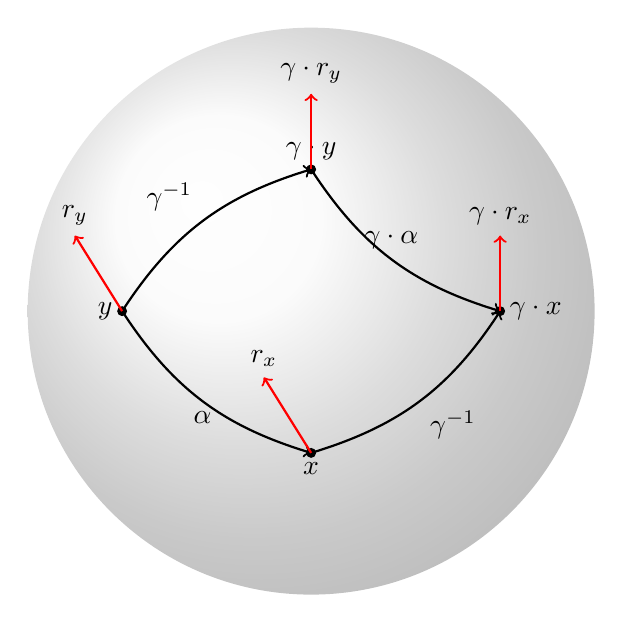
\begin{tikzpicture}[scale=1.2]
    % 背景球体效果
    \shade[ball color=gray!10, opacity=0.4] (0,0) circle (3cm);
    
    % 定义坐标
    \coordinate (X) at (0, -1.5);
    \coordinate (Y) at (-2, 0);
    \coordinate (gX) at (2, 0);
    \coordinate (gY) at (0, 1.5);
    
    % 画点
    \fill (X) circle (1.5pt) node[below] {$x$};
    \fill (Y) circle (1.5pt) node[left] {$y$};
    \fill (gX) circle (1.5pt) node[right] {$\gamma \cdot x$};
    \fill (gY) circle (1.5pt) node[above] {$\gamma \cdot y$};
    
    % 画路径
    \draw[thick, ->] (Y) to[bend right=20] node[below] {$\alpha$} (X);
    \draw[thick, ->] (gY) to[bend right=20] node[above] {$\gamma \cdot \alpha$} (gX);
    \draw[thick, ->] (Y) to[bend left=20] node[above left] {$\gamma^{-1}$} (gY);
    \draw[thick, ->] (X) to[bend right=20] node[below right] {$\gamma^{-1}$} (gX);
    
    % 画标架向量 (红色箭头)
    \draw[thick, red, ->] (Y) -- ++(-0.5, 0.8) node[black, above] {$r_y$};
    \draw[thick, red, ->] (X) -- ++(-0.5, 0.8) node[black, above] {$r_x$};
    \draw[thick, red, ->] (gY) -- ++(0, 0.8) node[black, above] {$\gamma \cdot r_y$};
    \draw[thick, red, ->] (gX) -- ++(0, 0.8) node[black, above] {$\gamma \cdot r_x$};
\end{tikzpicture}
\end{center}

现在设 $r_y$ 是 $R_H$ 在另一点 $y$ 处的标架。如上图所示，我们可以选取一条从 $y$ 到 $x$ 的路径 $\alpha$。我们将 $r_y$ 沿 $\alpha$ 平行移动得到 $x$ 处的标架 $r_x$。
由于 $r_y$ 和 $\gamma \cdot r_y$ 来自底流形 $X$ 上同一点的同一个标架，对于 $r_x$ 和 $\gamma \cdot r_x$ 也同理；且由于 $\alpha$ 和 $\gamma \cdot \alpha$ 来自 $X$ 上同一条路径，我们知道 $\gamma \cdot r_x$ 来自于 $\gamma \cdot r_y$ 沿 $\gamma \cdot \alpha$ 的平行移动。
这意味着 $\varphi(\gamma \cdot r_x) = \varphi(\gamma \cdot r_y)$ 且 $\varphi(r_x) = \varphi(r_y)$。因此 $g_\gamma(r_y) = g_\gamma(r_x)$。
\end{proof}

\begin{proposition}\label{periodinvariant}
周期映射在表示 $\rho$ 下是等变的，即 $\mathcal{P}(\gamma \cdot x) = \rho(\gamma) \cdot \mathcal{P}(x)$。
\end{proposition}

\begin{proof}
\[ \mathcal{P}(\gamma \cdot x) = \varphi_{P_H}(\gamma \cdot x) = \varphi(\gamma \cdot P_H(x)) = \rho(\gamma) \cdot \varphi(P_H(x)) = \rho(\gamma) \cdot \mathcal{P}(x) \]
\end{proof}

\subsection{Hodge表示与稳定性}

设 $V = \oplus_{p+q=k} V^{p,q}$ 为具有极化Hodge结构的复向量空间。

\begin{definition}
极化Hodge表示 $\Pi: G_0 \to \text{GL}(V)$ 是一个复表示，使得 $K_0$ 的作用保持Hodge分解，且 $\g$ 的作用与Hodge类型兼容（即 $\g^{k, -k} \cdot V^{p,q} \subset V^{p+k, q-k}$），并且半线性形式 $s$ 被 $G_0$ 保持。
\end{definition}

特别地，伴随表示 $\Ad: G_0 \to \text{GL}(\g)$ 是极化Hodge表示。

\begin{definition}
假设 $X$ 是紧致的，一个Hodge丛主系统 $(P, \theta)$ 称为 $\Pi$-稳定的，如果Hodge丛系统 $P \times_K V$ 是稳定的。
\end{definition}

对于非紧情况，我们需要选择度量 $P_H$ 使得 $\Lambda F_{\nabla^{hs}}$ 有界。

\begin{lemma}
设 $\Pi: G_0 \to V$ 为极化Hodge表示，如果 $\Lambda F_{\nabla^{hs}}$ 有界，则 $\Lambda {}^V F_{\nabla^{hs}}$ 也有界。
\end{lemma}

\begin{definition}
假设 $X$ 非紧，令 $(P, \theta, P_H)$ 为带有度量 $P_H$ 的Hodge丛主系统，满足 $\Lambda F_{\nabla^{hs}}$ 有界。我们称 $(P, \theta, P_H)$ 是 $(\Pi, P_H)$-稳定的，如果Hodge丛系统 $P \times_K V$ 关于度量 $(P_H, H)$ 是解析稳定的。
\end{definition}

\subsection{主 VHS 的构造}

我们有如下由 Simpson 得到的结果。

\begin{theorem}\label{prop8.1}
如果 $(P, \theta, P_H)$ 关于某个不可约极化Hodge表示族 $\{\Pi_i\}_i$ 是 $(\Pi_i, P_H)$-稳定的，且该表示族忠实地表示了 $\g$，即 $\oplus_i d\Pi_i$ 是单射，那么存在一个度量 $P_K$ 使得 $\Lambda F_{\nabla^{hs}} = 0$。如果此外 $X$ 是紧致的且 $c_2(P \times_K \g) \cdot [\omega]^{n-2} = 0$，则 $F_{\nabla^{hs}} = 0$，因此这给出了一个主Hodge结构形变。
\end{theorem}

\begin{proof}
固定一个初始度量 $P_{H_0}$ 使得解析稳定性的概念是良定义的。如果 $\Pi$ 是上述 $G_0$ 到 $(V, H) = (\oplus V_i, \oplus H_i)$ 的表示，那么 $H$ 和 $P_{H_0}$ 共同给出了 $P \times_K V = \mathcal{V} = \oplus \mathcal{V}_i$ 上的一个度量 $H_0$，这是一个 Hodge 丛系统的直和，或者说是具有 $U(1) \times U(1)$ 对称性的 Higgs 丛。此时我们可以调用定理~\ref{th1} 来运行 H-Y-M 流：
\[ h^{-1}\dot{h} = -\sqrt{-1}\Lambda F_{\nabla^{hs}_{H(t)}} \]
其中 $H(t) = H_0h$。由于曲率保持 $U(1) \times U(1)$ 对称性且解是唯一的，$h(t)$ 也保持该作用，特别是 $h$ 保持Hodge分解。稳定性条件给出了一个极限 $h_\infty$。为了证明 $h_\infty$ 来自于一个度量 $P_K$，只需证明对任意 $x$，有 $h_\infty(x) \in \Pi(K)$。为此，我们需要用到 Tannakian 范畴理论中的以下定理。

\begin{theorem}[Chevalley]
$GL(V)$ 的任意代数子群 $G$ 均可作为由 $V$ 的张量积、直和及对偶构成的向量空间 $T(V)$ 中一维子空间的稳定子出现。
\end{theorem}

或者等价地，我们可以将 $G$ 刻画为由 $V$ 和 $V^*$ 中的元素组成的有限个张量的稳定子。在我们的情形下，$\Pi(G)$ 由一组张量刻画。因此只需证明给定这样一个张量 $w$，有 $h(t) \cdot w = w$。由于 $w$ 是 $\Pi(G)$ 不变的，故 $\g \cdot w = 0$。

假设 $w \in T(V) \otimes T(V^*)$，令 $\mathcal{W}$ 为关联于由 $w$ 张成的线性子空间的线丛，$\mathcal{T}$ 为关联于 $T(V) \otimes T(V^*)$ 的丛，且 $\otimes h$ 为 $\mathcal{T}$ 上热方程的解。由于 $\Lambda F_0$ 是 $\g$-值的，故 $\Lambda F_0 \cdot w = 0$。于是由热方程解的唯一性可知 $\otimes h|_{\mathcal{W}} = \id$。另一方面，热方程的解与张量及对偶表示是兼容的，我们有 $h \cdot w = \otimes h \cdot w = w$。从而我们证明了 $h \in \Pi(G)$。

但我们知道 $h$ 保持Hodge分解，于是 $\Ad(h)\g^{p,-p} = \g^{p,-p}$（由于表示在李代数层面上是忠实的，我们将 $\g$ 的像与 $\g$ 等同）。由于 $K$ 根据定义是稳定Hodge结构的极大子群，我们有 $h \in \Pi(K)$，因此 $H_\infty$ 来自于 $K$-丛 $P$ 的一个 $K_0$-约化 $P_{H_\infty}$。稳定性条件表明 $\Lambda F_{\nabla^{hs}_{H_\infty}} = 0$，由于表示在李代数层面上是忠实的，我们在主丛上有 $\Lambda F_{\nabla^{hs}} = 0$。

如果 $X$ 紧致且 $c_2(P \times_K \g) \cdot [\omega]^{n-2} = 0$，则 $c_2(P \times_K V) \cdot [\omega]^{n-2} = 0$。事实上，由于 $\g$ 半单，$\g$ 上由 Ad-不变双线性对称形式张成的线性空间是一维的，因此 $c_2(P \times_K V) = C \cdot c_2(P \times_K \g)$，其中 $C$ 为常数。然后我们可以应用命题~\ref{prop3.3} 来证明 $F_{\nabla^{hs}} = 0$。
\end{proof}
\subsection{一个例子}

令 $V = \oplus V^{p,q}$ 为具有不定 Hermitian 形式 $s$ 的极化Hodge结构。定义 $G_0 := \Au(V, s)/U(1)$，则 $K_0 = \Au(V, h)/U(1)$。$G_0$ 是单李群，复化李代数 $\g = \En(V)^\perp$。$G_0$ 是极化Hodge群。

\begin{definition}
以 $V$ 为模型的射影 VHS 是一个主 VHS $(P_H, \nabla^{hs})$。
\end{definition}

\begin{lemma}\label{lemmabundletovhs}
假设 $X$ 紧致。如果Hodge丛系统 $E = \oplus E^{p,q}$ 是具有相同斜率的稳定丛的直和，并满足命题~\ref{prop3.3} 中的等式，则它诱导一个主 VHS。周期映射的微分是 $\theta: T(\tilde{X}) \to \En(E)^{-1, 1}$。
\end{lemma}
\begin{proof}
固定一个纤维，记为 $V$。来自 $E^{p,q}$ 的全纯标架模掉等价关系 $e \sim z \cdot e$ 给出了一个 $K$-torsor，即一个全纯主 $K$-丛，其中 $K = (\En(V)^\perp)^{0,0}$。Higgs 场给出了一个 $\En(V)^{-1,1}$-值的张量形式 $\theta$。
由于 $E$ 是多重稳定的（poly-stable），我们可以运行 H-Y-M 流并利用定理~\ref{th1} 和命题~\ref{prop3.3} 在 $E$ 上得到一个度量 $H$，使得 $F^\perp_{\nabla^{hs}_H} = 0$。
于是，射影酉标架给出了一个具有零曲率的 $K_0$-torsor（即一个度量）。
\end{proof}

\begin{corollary}\label{examplecor}
假设 $\mathcal{L}$ 是Hodge流形 $X$（带极化 $\Theta$）上的线丛，且存在非零态射 $\psi: \mathcal{L} \to \Omega_X^1$。如果 $\mathcal{L} \cdot \Theta^{n-1} > 0$，则 $\mathcal{L} \cdot \Theta^{n-2} \le 0$；若此外等号成立，则存在非平凡表示 $\pi_1(X) \to \text{PSL}(2, \mathbb{R})$ 以及从 $\tilde{X}$ 到上半平面的等变映射。
\end{corollary}

\begin{proof}
考虑丛 $\mathcal{L} \oplus \mathcal{O}_X$，将 $\mathcal{O}_X$ 视为 $(0, 1)$ 分量，$\mathcal{L}$ 视为 $(1, 0)$ 分量。定义 Higgs 场 $\theta = \begin{pmatrix} 0 & 0 \\ \psi & 0 \end{pmatrix}$。这是一个稳定的Hodge丛系统。利用命题~\ref{prop3.3}和上述引理，当等号成立时，得到 $G_0 = \text{PSU}(1, 1)$ 和 $K_0 \cong U(1)$ 的射影 VHS。齐性空间 $G_0/K_0 \cong \mathbb{H}$（上半平面）。
\end{proof}
\subsection{单值化 (Uniformization)}

\subsubsection*{Hermitian 对称空间}

\begin{definition}
Hermitian 类型的Hodge群是指类型为 $\mathfrak{g} = \mathfrak{g}^{0,0} \oplus \mathfrak{g}^{-1,1} \oplus \mathfrak{g}^{1,1}$ 且没有紧致因子的Hodge群。对于这样的群，$K_0$ 成为极大紧子群。齐性空间 $G_0/K_0$ 是非紧类型的 Hermitian 对称空间。
\end{definition}

实际上，以下三个概念是等价的：
\begin{center}
\begin{tikzpicture}[>=stealth, node distance=2cm, auto]
    % 定义节点
    \node (A) at (0, 2) {$G_0/K_0$};
    \node (B) at (-3, 0) {有界对称域};
    \node (C) at (3, 0) {Hermitian 对称空间};
    
    % 定义连线箭头
    \draw[<->] (A) -- (B);
    \draw[<->] (A) -- (C);
    \draw[<->] (B) -- (C);
\end{tikzpicture}
\end{center}

\begin{definition}
$X$ 的单值化丛是一个Hodge丛主系统 $(P, \theta)$，使得
\[ \theta: T(X) \to P \times_K \mathfrak{g}^{-1,1} \]
是同构。
\end{definition}

值得注意的是，如果 $G_0$ 没有中心，则 $\Ad$ 是忠实的，那么该数据等价于 $T(X)$ 的结构群从 $\mathrm{GL}(n, \mathbb{C})$ 约化到 $K$，这里我们将 $K$ 与其伴随表示 $\Ad: K \to \mathrm{GL}(\mathfrak{g}^{-1,1})$ 的像等同，并将 $\mathrm{GL}(\mathfrak{g}^{-1,1})$ 与 $\mathrm{GL}(n, \mathbb{C})$ 等同。更确切地说，如果我们能指定 $T(X)$ 的一些标架，使得它们逐点构成一个 $K'$-torsor，其中 $K' = \Ad(K)$（对于某个无中心的 $G_0$ 的 $K$），并且 $K'$ 在标架上的右作用与 $K$ 在 $\mathfrak{g}^{-1,1}$ 上的伴随作用相同，那么我们可以从这些数据得到一个单值化丛。实际上，记标架丛为 $P$，如果我们通过 $\Ad$ 将 $K'$ 与 $K$ 等同，那么 $P$ 就是一个 $K$-丛，显然有
\[ T(X) \cong P \times_{\text{st}(K')} \mathfrak{g}^{-1,1} \cong P \times_K \mathfrak{g}^{-1,1}. \]

\begin{example}
假设 $T(X) = \oplus_{i=1}^n L_i$，其中 $L_i$ 为线丛。那么我们可以考虑保持该分解的标架，此时标架丛 $P$ 是一个 $K' = \mathbb{C}^{*n}$-丛。实际上，$K'$ 来自于与 Hermitian 类型Hodge群 $G_0 = \mathrm{PSU}(1,1)^n$ 关联的 $K$ 的伴随表示，其关联的有界对称域为 $\mathbb{D}^n$。
\end{example}

让我们详细讨论一下。令 $G_0 = \mathrm{PSU}(1,1)$。它看起来像
\[ \begin{pmatrix} \alpha & \beta \\ \bar{\beta} & \bar{\alpha} \end{pmatrix}, \quad |\alpha|^2 - |\beta|^2 = 1 \]
其李代数 $\mathfrak{su}(1,1)$ 有三个生成元
\[ \mathfrak{k}_0 = \begin{pmatrix} i & 0 \\ 0 & -i \end{pmatrix}, \quad \mathfrak{p}_1 = \begin{pmatrix} 0 & 1 \\ 1 & 0 \end{pmatrix}, \quad \mathfrak{p}_2 = \begin{pmatrix} 0 & i \\ -i & 0 \end{pmatrix} \]
其复化 $\mathfrak{g}$ 有三个生成元
\[ \mathfrak{g}^{0,0} = \begin{pmatrix} 1 & 0 \\ 0 & -1 \end{pmatrix} \]
\[ \mathfrak{g}^{-1,1} = \frac{1}{2}(\mathfrak{p}_1 - i\mathfrak{p}_2) = \begin{pmatrix} 0 & 1 \\ 0 & 0 \end{pmatrix}, \quad \mathfrak{g}^{1,-1} = \frac{1}{2}(\mathfrak{p}_1 + i\mathfrak{p}_2) = \begin{pmatrix} 0 & 0 \\ 1 & 0 \end{pmatrix} \]
并且
\[ K = \begin{pmatrix} z & 0 \\ 0 & z^{-1} \end{pmatrix} / \{\pm \id\} \cong \mathbb{C}^* / \{\pm \id\} \]
$K$ 在 $\mathfrak{g}^{-1,1}$ 上的伴随表示是乘以 $z^2$。因此表示 $K'$ 的像仍然是 $\mathbb{C}^*$。

\begin{example}[典范 Higgs 丛]
设 $X$ 是紧致的，丛 $\Omega_X^1 \oplus \mathcal{O}_X$ 连同 $\theta = T(X) \cong \mathrm{Hom}(\Omega_X^1, \mathcal{O}_X)$ 被称为典范 Higgs 丛。如果它容许一个度量使得 $F_{\nabla^{ns}}^\perp = 0$，那么它是一个 $G_0 = \mathrm{PU}(n,1)$ 的单值化形变。
\end{example}

这直接由引理~\ref{lemmabundletovhs}得出。$\mathrm{PU}(n,1)$ 是 Hermitian 类型的Hodge群，其关联的有界对称域是单位球 $\mathbb{B}^n$。其Hodge类型如下：
\[ \mathfrak{g}^{0,0} = \left\{ \begin{pmatrix} A & 0 \\ 0 & -\mathrm{tr}(A) \end{pmatrix} \middle| A \in M_n(\mathbb{C}) \right\} \]
\[ \mathfrak{g}^{-1,1} = \left\{ \begin{pmatrix} 0 & v \\ 0 & 0 \end{pmatrix} \middle| v \in \mathbb{C}^n \right\} \quad \mathfrak{g}^{1,-1} = \left\{ \begin{pmatrix} 0 & 0 \\ w & 0 \end{pmatrix} \middle| w \in (\mathbb{C}^n)^T \right\}. \]

\subsubsection*{单值化 VHS}

单值化Hodge结构形变是带有一个平坦度量 $P_H$ 的单值化丛 $(P, \theta)$。

\begin{proposition}
设 $X$ 是完备 Kähler 流形，$\tilde{X}$ 为其万有覆叠。则 $\tilde{X}$ 同构于有界对称域 $\mathcal{D}$ 当且仅当存在一个关于某个满足 $\mathcal{D} = G_0/K_0$ 的Hodge群 $G_0$ 的单值化 VHS，且 $\theta^{-1}$ 有界。
\end{proposition}

\begin{proof}
假设存在这样的单值化形变。由于 $\theta$ 是周期映射 $\mathcal{P}$ 的微分，它是一个局部微分同胚。因为它是 $\pi_1(X)$-等变的，我们可以证明 $\mathcal{P}$ 是闭映射，因此是满射。由于 $dP^{-1} = \theta^{-1}$ 有界且 $\tilde{X}$ 完备，易证 $\mathcal{P}$ 是覆叠映射。但由于 $\mathbb{D}$ 是单连通的，故 $\mathcal{P}$ 是同构。

反之，如果 $\tilde{X} \cong \mathbb{D}$ 且它是 $\pi_1(X)$ 等变的。令 $G_0$ 为 $\mathbb{D}$ 的全纯自同构群，则 $\mathbb{D} \cong G_0/K_0$，$\pi_1(X)$ 通过全纯自同构作用于 $\mathbb{D}$，因此我们得到了一个表示。只需在 $\mathbb{D}$ 上构造一个主 VHS，它是自然产生的。我们将 $G_0$ 视为 $\mathbb{D}$ 上的主 $K_0$-丛，根据 Cartan 分解，其 Cartan-Maurer 形式 $\omega = g^{-1}dg$ 分解为 $\omega_{\mathfrak{k}}$ 和 $\omega_{\mathfrak{h}}$，前者是联络形式，后者是张量形式。我们有 $d\omega + \frac{1}{2}[\omega, \omega] = 0$。将 $G_0$ 的结构群扩张到 $K$，得到 $P = G_0 \times_{K_0} K$。$\omega_{\mathfrak{h}}$ 分裂为 $\omega_{\mathfrak{h}^-}$ 和 $\omega_{\mathfrak{h}^+}$。由于曲率 $\Omega_{\mathfrak{k}} = d\omega_{\mathfrak{k}} + \frac{1}{2}[\omega_{\mathfrak{k}}, \omega_{\mathfrak{k}}] = -\frac{1}{2}[\omega_{\mathfrak{h}}, \omega_{\mathfrak{h}}]$，这意味着曲率的 $(0,2)$ 部分消失，因此 $\omega_{\mathfrak{k}}$ 的 $(0,1)$ 部分给出了 $P$ 上的全纯结构，$\omega_{\mathfrak{h}^-}$ 是一个 Higgs 场。如果我们进一步将这些结构扩张到 $R_H = G_0 \times_{K_0} G_0$，那么 $\omega$ 就是我们想要的平坦 Hitchin-Simpson 联络。

我们甚至可以检查周期映射是什么！实际上，很容易看出 $[g, g^{-1}]$ 是关于 $\omega$ 的平坦截面，因此周期映射是恒等映射 $\id$。
\end{proof}

\subsubsection*{单值化丛的稳定性}

将 $\mathfrak{g}$ 分解为单理想 $\mathfrak{g} = \oplus \mathfrak{g}_i$。它们是子Hodge结构，如果 $G_0$ 是连通的，它们是 $G_0$ 的Hodge表示。为了更一般化，我们不假设连通性。如果 $(P, \theta)$ 是单值化丛，局部上我们可以将 $P \times_K \mathfrak{g}$ 分解为 $\oplus \mathfrak{g}_i$，但全局上它们被 $G$ 的伴随表示扭曲。然而，我们可以找到 $P \times_K \mathfrak{g}$ 的唯一最细全局分解 $\oplus U_j$，使得 $U_j$ 局部上是 $\{\mathfrak{g}_i\}_i$ 的固定子集的直和，即单李代数集合分解为不相交的子集 $\mathfrak{u}_j$。$U_j$ 可能不来自 $G$ 的表示，但我们可以找到 $G$ 的子群 $G'$ 使得 $P$ 的结构群可以约化为 $K' = K \cap G'$，且 $U_j = P' \times_{K'} \mathfrak{u}_j$，同时整个伴随丛的全纯结构被保持，即 $P \times_K \mathfrak{g} \cong P' \times_{K'} \mathfrak{g}$。如果需要，我们将始终假设已进行此类约化。

\begin{definition}
一个单值化丛是稳定的，如果它对所有 $j$ 都是 $\mathfrak{u}_j$-稳定的。
\end{definition}

调用一个关于李代数的引理。

\begin{lemma}
假设 $\mathfrak{g}_0$ 是我们考虑类型的单李代数。如果 $e \in \mathfrak{g}^{-1,1}$，则
\[ [\mathfrak{g}^{-1,1}, [\mathfrak{g}^{-1,1}, e]] = \mathfrak{g}^{-1,1}. \]
\end{lemma}

\begin{corollary}
假设 $\mathfrak{g}$ 是半单的。如果 $W \subset \mathfrak{g}$ 是一个子Hodge结构使得 $[\mathfrak{g}^{-1,1}, W] \subset W$，则 $\dim W^{-1,1} \ge \dim W^{1,-1}$。如果等号成立，则 $W$ 是 $\mathfrak{g}$ 的理想的直和。
\end{corollary}

\begin{corollary}
假设 $(P, \theta)$ 是单值化Hodge丛系统。则以下条件等价：
\begin{enumerate}
    \item $(P, \theta)$ 是稳定的。
    \item $P \times_K \mathfrak{g}$ 是度数为零的稳定系统的直和。
    \item $P \times_K \mathfrak{g}$ 的每个满足 $\deg(W) \ge 0$ 的饱和Hodge层子系统 $W$ 局部上是某些 $\mathfrak{g}_i$ 的直和。
\end{enumerate}
\end{corollary}

\begin{proof}
1. $\Rightarrow$ 2. 写出 $P \times_K \mathfrak{g} = U_j$，则 $U_j$ 是稳定的，且由于 $\mathfrak{u}_j$ 是半单的，它的度数为零。
2. $\Rightarrow$ 3. 由于 $P \times_K \mathfrak{g}$ 是多重稳定的 (polystable)，$\deg W = 0$ 且 $P \times_K \mathfrak{g} = W \oplus W'$。特别地，$W'$ 也是Hodge丛系统。对 $W$ 和 $W'$ 应用上一个推论，两者均等号成立。
3. $\Rightarrow$ 1. 如果 $W \subset U_j$ 是满足 $\deg W \ge 0$ 的饱和Hodge层子系统，则 $W$ 局部上是某些 $\mathfrak{g}_i$ 的直和，因为 $U_j$ 是最细的，所以 $W = U_j$。
\end{proof}

\begin{theorem}
假设 $X$ 是紧致的。$\tilde{X} \cong \mathbb{D}$ 当且仅当存在一个结构群 $G_0$ 对应于 $\mathbb{D}$ 的单值化丛 $(P, \theta)$，使得 $(P, \theta)$ 是稳定的且 $c_2(P \times_K \mathfrak{g}) \cdot [\omega]^{n-2} = 0$。
\end{theorem}

\begin{proof}
每个 $U_j$ 来自 $G'$ 到 $\mathfrak{u}_j$ 的不可约Hodge表示。应用定理 9 我们知道 $(P, \theta)$ 是单值化 VHS。应用命题 13 我们知道 $\tilde{X} \cong \mathbb{D}$。反之，应用命题 13 我们得到单值化 VHS $(P, \theta)$。因此 $P \times_K \mathfrak{g}$ 的所有陈类消失，且它是多重稳定的。应用上述推论，我们知道 $(P, \theta)$ 是稳定的。
\end{proof}

\begin{corollary}
设 $\mathbb{D}$ 如前所述，设 $X$ 是光滑射影簇。则对于任意 $\sigma \in \Au(\mathbb{C}/\mathbb{Q})$，如果 $X$ 被 $\mathbb{D}$ 单值化，那么 $X^\sigma$ 也是。
\end{corollary}

\begin{proposition}
假设 $X$ 是紧致的且 $(P, \theta)$ 是单值化丛。则
\[ \theta: T(X) \cong P \times_K \mathfrak{g}^{-1,1} \cong \oplus_j V_j. \]
如果 $V_j$ 是半稳定的且度数严格小于零，则 $(P, \theta)$ 是稳定的。因此如果 $c_2(P \times_K \mathfrak{g}) \cdot [\omega]^{n-2} = 0$，则 $(P, \theta)$ 是 $X$ 的单值化 VHS。
\end{proposition}

\begin{proof}
假设 $G$ 是连通的。则 $K$ 在 $\mathfrak{g}_i^{-1,1}$ 上的作用是不可约的，因此 $V_i = P \times_K \mathfrak{g}_i^{-1,1}$。$P \times_K \mathfrak{g}_i^{-1,1}$ 和它们的对偶 $P \times_K \mathfrak{g}_i^{1,-1}$ 是半稳定的。李括号
\[ [\cdot, \cdot]: P \times_K \mathfrak{g}_i^{-1,1} \otimes P \times_K \mathfrak{g}_i^{1,-1} \to P \times_K \mathfrak{g}_i^{0,0} \]
是满射，因此右边是度数为零的半稳定的。假设 $W \subset P \times_K \mathfrak{g}_i$ 是Hodge层子系统。则 $\deg(W^{0,0}) \le 0$ 且 $\deg(W^{1,-1}) \le -\mathrm{rank}(W^{1,-1}) \cdot \mu$ 以及 $\deg(W^{-1,1}) \le \mathrm{rank}(W^{1,1}) \cdot \mu$，其中 $\mu(V_i) < 0$ 是斜率。因此
\[ \mu(W) \le (\mathrm{rank}(W^{-1,1}) - \mathrm{rank}(W^{1,-1})) \cdot \mu(V_i) \le 0 \]
如果等号成立，则利用推论 15 可知 $W=V_i$，因此 $V_i$ 是稳定的。

假设 $G$ 不连通。令 $G^o$ 为 $G$ 的连通分支，$K^o$ 为 $K$ 的连通分支。则 $P/K^o$ 是一个 $K/K^o$-主丛，它也是 $X$ 的覆叠空间。我们有单值性 (monodromy) $\pi_1(X) \to K/K^o$。找一个覆叠 $\pi: X^o \to X$，其基本群是单值性的核，那么我们可以在 $X^o$ 上将 $P$ 的结构群从 $K$ 约化到 $K^o$。拉回 $\pi^*(V_j)$ 是半稳定的。如果我们关于 $K^o$ 作用分解 $TX^o = \oplus V_k^o$，则 $\pi^*(V_j)$ 是某些 $V_k^o$ 的直和。因此每个 $V_k^o$ 都是负度数半稳定的。根据上述关于连通 $G^o$ 的讨论，它们是稳定的，因此 $P \times_K \mathfrak{g} = P^o \times_{K^o} \mathfrak{g}$ 在 $X^o$ 上是多重稳定的。如果 $W$ 是 $X$ 上满足 $\deg(W) \ge 0$ 的Hodge层子系统，那么它的拉回 $\pi^*W$ 具有零度数，必定是 $P^o \times_{K^o} \mathfrak{g}$ 的稳定子丛的直和。因此由推论 15，它是单理想的局部直和，对于 $W$ 也是如此，因此由推论 16，$(P, \theta)$ 是稳定的。
\end{proof}

\begin{corollary}
假设 $X$ 是紧致的。如果 $T_X = \oplus_{i=1}^n L_i$ 是负度数线丛的直和，并且 $(c_1(X)^2 - 2c_2(X)) \cdot [\omega]^{n-2} = 0$，则 $X$ 被 $\mathbb{B}^n$ 单值化。
\end{corollary}

\begin{proof}
由例 1 的讨论可知，我们有一个 $K = (\mathbb{C}^*/\{\id, -\id\})^n$ 的单值化丛。其关联的有界对称域是 $\mathbb{B}^n$。直接计算表明 $c_2(P \times_K \mathfrak{g}) = 2c_2(X) - c_1(X)^2$。
\end{proof}

接下来调用例 2 中的典范 Higgs 丛 $W$。

\begin{proposition}[Miyaoka-Yau 不等式]
假设 $X$ 是紧致的。如果 $W$ 是稳定的，则
\[ \left( 2c_2(X) - \frac{n}{n+1} c_1(X)^2 \right) \cdot [\omega]^{n-2} \ge 0 \]
如果等号成立，则 $X$ 被 $\mathbb{B}^n$ 单值化。
\end{proposition}

如果 $X$ 是紧致曲线，则陈类条件平凡成立，$W$ 稳定当且仅当 $X$ 的亏格 $g$ 大于 2。因此，如果 $g \ge 2$，$X$ 被 $\mathbb{B}$ 单值化，这就是经典的单值化。

\begin{proposition}
假设 $X$ 是紧致 Kähler 曲面。如果 $c_1(X)^2 \ge 3c_2(X)$，$c_1(X)^2 \ge 0$ 且 $c_1(X) \cdot [\omega] < 0$，则 $W$ 是稳定的，从而 $c_1(X)^2 = 3c_2(X)$ 且 $\tilde{X} = \mathbb{B}^2$。
\end{proposition}

\begin{proof}
只需证明对偶 Higgs 丛 $W^* = (\mathcal{O}_X, T_X)$ 是稳定的。秩为 2 的唯一饱和子层是 $T_X$，由 $c_1(X) \cdot [\omega] < 0$ 满足条件。秩为 1 的饱和子层是 $T_X$ 的可逆子层，它们在有限集之外是线子丛。设 $L$ 为这样的子层。我们必须证明 $c_1(L) \cdot [\omega] < \frac{1}{3} c_1(X) \cdot [\omega]$。反之假设不成立。令 $M = T_X/L$，它是余维数 1 的线丛。令 $N = M^{**}$，则它是线丛，且 $M \hookrightarrow N$ 的商支集在有限集上。$(\mathcal{O}_X, N)$ 是一个Hodge丛系统，且
\[ c_1(N) \cdot [\omega] \le \frac{2}{3} c_1(X) \cdot [\omega] \le 0 \]
因此它是稳定的。B-G 不等式蕴含 $c_1(N)^2 \le 0$。在 Grothendieck 群中 $T_X$ 等于 $N + L - (N/M)$，因此
\[ \begin{aligned} c_2(X) &= c_1(N)c_1(L) - c_2(N/M) \\ &= c_1(X)c_1(N) - c_1(N)^2 - c_2(N/M) \\ &\ge c_1(N)c_1(X) - c_1(N) \end{aligned} \]
最后一个不等式成立是因为 $c_2(N/M)$ 等于其支集中点的非正和。因此
\[ (c_1(N) - 2c_1(X))^2 \ge 4(c_1(X)^2 - 3c_2(X)) \ge 0 \]
由我们的假设。另一方面，我们将Hodge指数定理应用于 $H^{1,1}(X, \mathbb{R})$。其上的相交形式具有符号 $(1, h^{1,1}-1)$，我们可以选择由 $\omega$ 张成的正定子空间。因此 $c_2(X)$ 位于正锥的负半部的内部，而 $3c_1(N)$ 在 $2c_1(X)$ 下方的锥外。因此 $3c_1(N) - 2c_1(X)$ 严格在锥外，所以它的平方严格为负，导致矛盾。
\end{proof}
\subsection{非紧曲线上的Hodge丛}
令$X$为一个非紧黎曼面，$\overline{X}$为$X$的一个光滑紧化，令$\omega$为$\overline{X}$上的一个 K\"ahler 形式，其在$X$上的限制依然记为$\omega$。令$j:X\to \overline{X}$为其嵌入映射，令$Y=\overline{X}-X$. 
\begin{definition}\label{regularsytemofhodgebundle}
    一个$X^{alg}$上的\textbf{正则Hodge丛}是一个代数Hodge丛$E$并存在以下尊重Hodge分解的滤链：
    \[
    j_*^{alg}E=\bigcup_{\alpha\in \R^{Y}} E_{\alpha}
    \]
其中$E_\alpha$皆为凝聚子层，我们赋予$\R^{Y}$自然的偏序结构，我们要求该滤链关于偏序结构是左连续并且递降的。并且我们要求Higgs场满足
\[
\theta: E^{p,q}_\alpha \to E^{p-1,p+1}_\alpha\otimes \Omega_X^1\langle\log(Y)\rangle
\]
\end{definition}
下面我们会看到这样的定义是自然的。假设我们有一个全纯的Hodge丛$E\to X$，如果$E$上存在一个在奇点附近行为较好的和Hodge结构相容的度量$h$ （我们总是假设度量和Hodge结构相容），我们可以通过如下方式构造出一族子层$a_hE^{p,q}=\bigcup_{\alpha\in \R^{Y}} E^{p,q}_\alpha$：我们定义$E^{p,q}_\alpha$为$j^{an}_*E^{p,q}$当中满足以下条件的子层，对任意的$y\in Y$，假设$y\in\U$，我们只选取增长速度满足
\[
|s|_h\leq C r^{\alpha_y-\epsilon},\quad \text{对充分小的}\epsilon>0
\]
的那些截面$s$。

Simpson\cite{Si1}证明了以下定理，
\begin{theorem}
    假设$(E,\overline{\partial},\theta, h)$是一个带度量的Hodge丛，并且度量$h$满足
    \[
    \int_X |F_{\nabla^{hs}_h}|^p <\infty,\quad p>1
    \]
    则如上定义的$E_\alpha$是凝聚层，并且$\theta$满足
    \[
    \theta: E^{p,q}_\alpha \to E^{p+1,q-1}_\alpha \otimes \Omega_X^1\langle\log Y\rangle
    \]
    因此$E$是一个正则Hodge丛。上述的构造 $a$ 和取行列式，对偶，张量积可交换。如果$h$和$h'$两个度量满足$a_h=a_h'$，那$h$和$h'$是可比的。并且我们有$a$作为从带$L^p$--曲率度量的Hodge丛打到正则Hodge丛的函子，它是一个范畴等价。
\end{theorem}

我们先证明以下引理：

\begin{lemma}\label{boundofHiggs}
    对于Hodge丛$(E,\overline{\partial},\theta)$，固定某个$p>1$。对任意的度量$h$满足
    \[
    \int_X |F_{\nabla^{hs}_{h}}|^p<\infty,
    \]
    则Higgs场满足
    \[
    \sup |\theta|\leq \frac{C}{|z\log|z||}
    \]
    这里$z$是某个$y\in Y$附近的一个小坐标邻域，常数$C$被曲率的$L^p$--范数所决定。
\end{lemma}
\begin{proof}
   不妨给坐标邻域赋予标准欧式度量。因此张量丛$(\En(E))^{-1,1}\otimes \Omega_X^1$的Chern曲率完全由$\nabla_h^2$的伴随作用给出，其中$\nabla_h$是丛$(E,\overline{\partial},h)$的Chern曲率张量。由于全纯子丛的曲率小于等于整体曲率的限制，因此如果我们把$\theta$看成$(\En(E))^{-1,1}\otimes \Omega_X^1$的一个线丛子丛的话，在$\theta$不为0处，我们有以下不等式
   \[
   \Delta \log|\theta|^2\leq \frac{\langle2i\ad\Lambda\nabla_h^2(\theta),\theta \rangle_h}{|\theta|^2}.
   \]

   令一方面，任给切向量$v\in T^{1,0}$，$\theta(v)$是周期域$G_0/K_0$的切向量，由\cite{griffiths1969locally}中的结论，周期域的全纯截面曲率在$\g^{-1,1}$方向上是严格负的，因此我们有
\[
\frac{R(\theta(v),\overline{\theta}(\bar{v}),\theta(v),\overline{\theta}(\bar{v}))}{|\theta(v)|^4}=-\langle [[\theta(v),\overline{\theta}(\bar{v})],\theta(v)],\theta(v)\rangle\leq -C
\]
取局部坐标$z$使得$\omega=\frac{i}{2}\diff z\wedge \diff \overline{z}$以及丛的酉标架。在此平凡化下
\[\theta=\phi\diff z, \quad \overline{\theta}=\phi^\dagger \diff \overline{z}\]
\[|\theta|^2=2\tr(\phi\phi^\dagger),\quad [\theta,\theta^\dagger]=(\phi\phi^\dagger-\phi^\dagger\phi)\diff z\wedge \diff \overline{z}\]
\[
i\Lambda[\theta,\theta^\dagger]=2(\phi\phi^\dagger-\phi^\dagger\phi)=2[\theta(\frac{\partial}{\partial z}), \overline{\theta}(\frac{\partial}{\partial \overline{z}})]=2[A,A^\dagger]\]

\[
   \langle [\frac{i}{2}\Lambda[\theta,\theta^\dagger],\theta],\theta\rangle=2\langle [[A,A^\dagger],A],A\rangle
\]
因此我们有
\[
\frac{\langle [2i\Lambda[\theta,\overline{\theta}],\theta],\theta\rangle}{|\theta|^2}\geq C|\theta|^2.
\] 
令$f$为一个在去心圆盘上的$L^p$光滑函数使得$|F_{\nabla^hs}|\leq f$。如果$\sigma$满足$\Delta\sigma=-f$。由椭圆正则性理论可知我们可以选取$\sigma$为有界连续函数，因此$e^{-\sigma}$也是有界的。我们不妨将$h$修改为$he^{-\sigma}$而它们是可比的，因此我们不妨假设$i\Lambda F_{\nabla^hs}$是负定的。然而我们有$F_{\nabla^{hs}}=\nabla_h^2-[\theta,\overline{\theta}]$。因此在$\theta$不为0处我们有
\[
\Delta\log|\theta|^2\leq -C|\theta|^2
\]
由于$\theta$趋于0时我们有$\log|\theta|^2\to -\infty$，因此上述不等式在分布意义下成立，故我们可以利用Ahlfors'引理得证。
\end{proof}
为了得到$E_{\alpha}$的凝聚性，我们需要调用一些Cornalba--Griffiths~\cite{cornalba1975analytic}当中的结果，我们称$A$为特殊仿射光滑代数簇，如果$A=\overline{A}-D$其中$\overline{A}$是光滑射影簇，$D=\cup_{i=1}^{N} D_i$是一个简单正规充沛的除子。$A$总是可以被有限个形如${\Delta^*}^k\times \Delta^{n-k}$的坐标邻域所覆盖，其中$\Delta$是单位圆盘，$\Delta^*$是去心单位圆盘。$A$上总是存在一个和Poincar\'e度量可比的K\"ahler度量我们记为$\omega_P=\diff\diff^c\tau$. 令$\sigma=\sigma_1\otimes\cdots \otimes \sigma_N$为除子$D$的典范截面。则\[\tau=C\log|\sigma|^{-2}-\log((\log|\sigma_1|^2)^2\cdots(\log|\sigma_N|^2)^2)\]
\begin{theorem}[pp.23]\label{GAGAforbundle}
    设$E$是一个特殊仿射光滑代数簇$A$上面的全纯向量丛，那么$E$是代数的当且仅当$E$上面存在度量$h$使得$|\nabla_h^2|_{h,\omega_P}<C$。
\end{theorem}
\begin{theorem}[pp.24]\label{GAGAforbundle2}
    如果$E$满足上述条件，\[H^0(A,E^{alg})=\{s\in H^0(A^{an},E^{an})|\int_A |s|^2e^{-N\tau}\omega_p^n< \infty\quad\text{对某些整数N成立}\}\]
\end{theorem}

回到主定理的证明，由上述引理中的讨论我们还可以得到\[|\nabla_h^2|\leq f+\frac{C}{||z|\log|z||^2}\]
虽然$|\nabla_h^2|$和Cornalba--Griffiths理论的要求相差了一个$f$，但是他们证明主要的技巧是通过修改$h$，使得$i\Lambda\nabla_h^2$变成负定算子。在我们的条件下，此方法依然奏效。令$\chi=\sigma-C\log\log|z|^{-1}$，将原始的度量修改为与其可比的度量$he^{-\chi}$。因此$i\Lambda\nabla_h^2$是负定的。因此我们依然可以运用以上定理到去心黎曼面的场景，通过简单的计算结合以上定理我们知道$E$是代数的并且其作为代数凝聚层
\[
\bigcup_\alpha E_\alpha = E^{alg}
\]
因此$E$可以紧化为$\overline{X}$上面的凝聚层$\overline{E}$，令$\{e_1,\cdots,e_r\}$为包含$y\in Y$的一个Zariski开集上的代数标架，则在包含$y$的单位圆盘上，$|e_i|_h<|z|^{\alpha_i+\epsilon}$。通过乘适当的$z^{k_i}$作调整，以及调整标架的顺序，我们不妨假设$0\leq\alpha_i\leq\alpha_{i+1}<1$，因此我们得到$y$处的抛物结构。因此$\overline{E}=E_0$。由此不难看出$E_\alpha$是$\overline{X}$上的局部自由层，并且对任意的$\alpha$，$E_\alpha$和$E_0$给出的抛物信息是一样的。

在局部坐标下$\theta=f_{ij}e_i\otimes e_j^* \otimes \diff z$，由引理~\ref{boundofHiggs}易知$f_{ij}$最多只能有一阶极点，因此我们证明了$\theta\in H^0(\En(E_\alpha)\otimes \Omega_{\overline{X}}\langle\log Y\rangle)$。由于$h$和$E$的Hodge结构是相容的，因此上述讨论对于分量$E_\alpha^{p,q}$依然成立。

% Lorem ipsum dolor sit amet, consectetur adipiscing elit, sed do eiusmod tempor
% incididunt ut labore et dolore magna aliqua.
% \footnote{Ut enim ad minim veniam, quis nostrud exercitation ullamco laboris
%   nisi ut aliquip ex ea commodo consequat.
%   Duis aute irure dolor in reprehenderit in voluptate velit esse cillum dolore
%   eu fugiat nulla pariatur.}
